\documentclass{beamer} 
\usepackage{beamerthemesplit} 
\usepackage{wrapfig} 
\usepackage{verbatim} 
\usetheme{SPbGU} 
\usepackage{pdfpages} 
\usepackage{amsmath} 
\usepackage{cmap}
\usepackage{array} 
\usepackage[T2A]{fontenc} 
\usepackage[utf8]{inputenc} 
\usepackage[english,russian]{babel} 
\usepackage{indentfirst} 
\usepackage{amsmath} 
\usepackage{tikz} 
\usepackage{multirow} 
\usepackage[noend]{algpseudocode} 
\usepackage{algorithm} 
\usepackage{algorithmicx} 
\usetikzlibrary{shapes,arrows} 
\usepackage{fancyvrb} 
\usepackage{tikz} 
\usepackage{pgfplots} 
\usepackage{sidecap} 
\usepackage{soul}
\usepackage{xcolor}
\usepackage{tabu}
\usepackage{tikz}
\usetikzlibrary{calc}
\usepackage{zref-savepos}
\usepackage{colortbl}
\usepackage[normalem]{ulem}
\pgfplotsset{compat=1.9} 
\newtheorem{rutheorem}{Теорема} 
\newtheorem{ruproof}{Доказательство} 
\newtheorem{rudefinition}{Определение} 
\newtheorem{rulemma}{Лемма} 
\beamertemplatenavigationsymbolsempty 

\newcounter{NoTableEntry}
\renewcommand*{\theNoTableEntry}{NTE-\the\value{NoTableEntry}}

\newcommand*{\strike}[2]{%
	\multicolumn{1}{#1}{%
		\stepcounter{NoTableEntry}%
		\vadjust pre{\zsavepos{\theNoTableEntry t}}% top
		\vadjust{\zsavepos{\theNoTableEntry b}}% bottom
		\zsavepos{\theNoTableEntry l}% left
		\hspace{0pt plus 1filll}%
		#2% content
		\hspace{0pt plus 1filll}%
		\zsavepos{\theNoTableEntry r}% right
		\tikz[overlay]{%
			\draw
			let
			\n{llx}={\zposx{\theNoTableEntry l}sp-\zposx{\theNoTableEntry r}sp-\tabcolsep},
			\n{urx}={\tabcolsep},
			\n{lly}={\zposy{\theNoTableEntry b}sp-\zposy{\theNoTableEntry r}sp},
			\n{ury}={\zposy{\theNoTableEntry t}sp-\zposy{\theNoTableEntry r}sp}
			in
			(\n{llx}, \n{lly}) -- (\n{urx}, \n{ury})
			;
		}% 
	}%
}

\title[]{Синтаксический анализ Shuffled Languages} 
% То, что в квадратных скобках, отображается в левом нижнем углу. 
\institute[СПбГУ]{ Санкт-Петербургский Государственный Университет } 

% То, что в квадратных скобках, отображается в левом нижнем углу. 
%\author[Горохов Артем]{Горохов Артем}
%\newline
%\textbf{Научный руководитель:} к.ф.-м.н., доцент Григорьев С.В.\newline
%\textbf{Рецензент:} программист СУИ НИУ ИТМО Авдюхин Д.А.} 
\author[Горохов Артем]{Горохов Артём В. \\
    \and  
    {\bfseries Руководитель:} Григорьев Семён В. \\
}
\date{16 декабря 2017} 

\begin{document} 
\definecolor{red}{RGB}{255,0,0} 

\begin{frame}
	\begin{center} 
		\begin{columns}
			\begin{column}{3cm}
			
\includegraphics[width=2cm]{pictures/SPbGU_Logo.png}
			
			\end{column}
			\begin{column}{3cm}
				 
\includegraphics[width=2cm]{pictures/jb.png}
				
			\end{column}
			\end{columns}	
	\end{center}
	\titlepage
\end{frame}



%\begin{frame}
%	\begin{center} 
%		{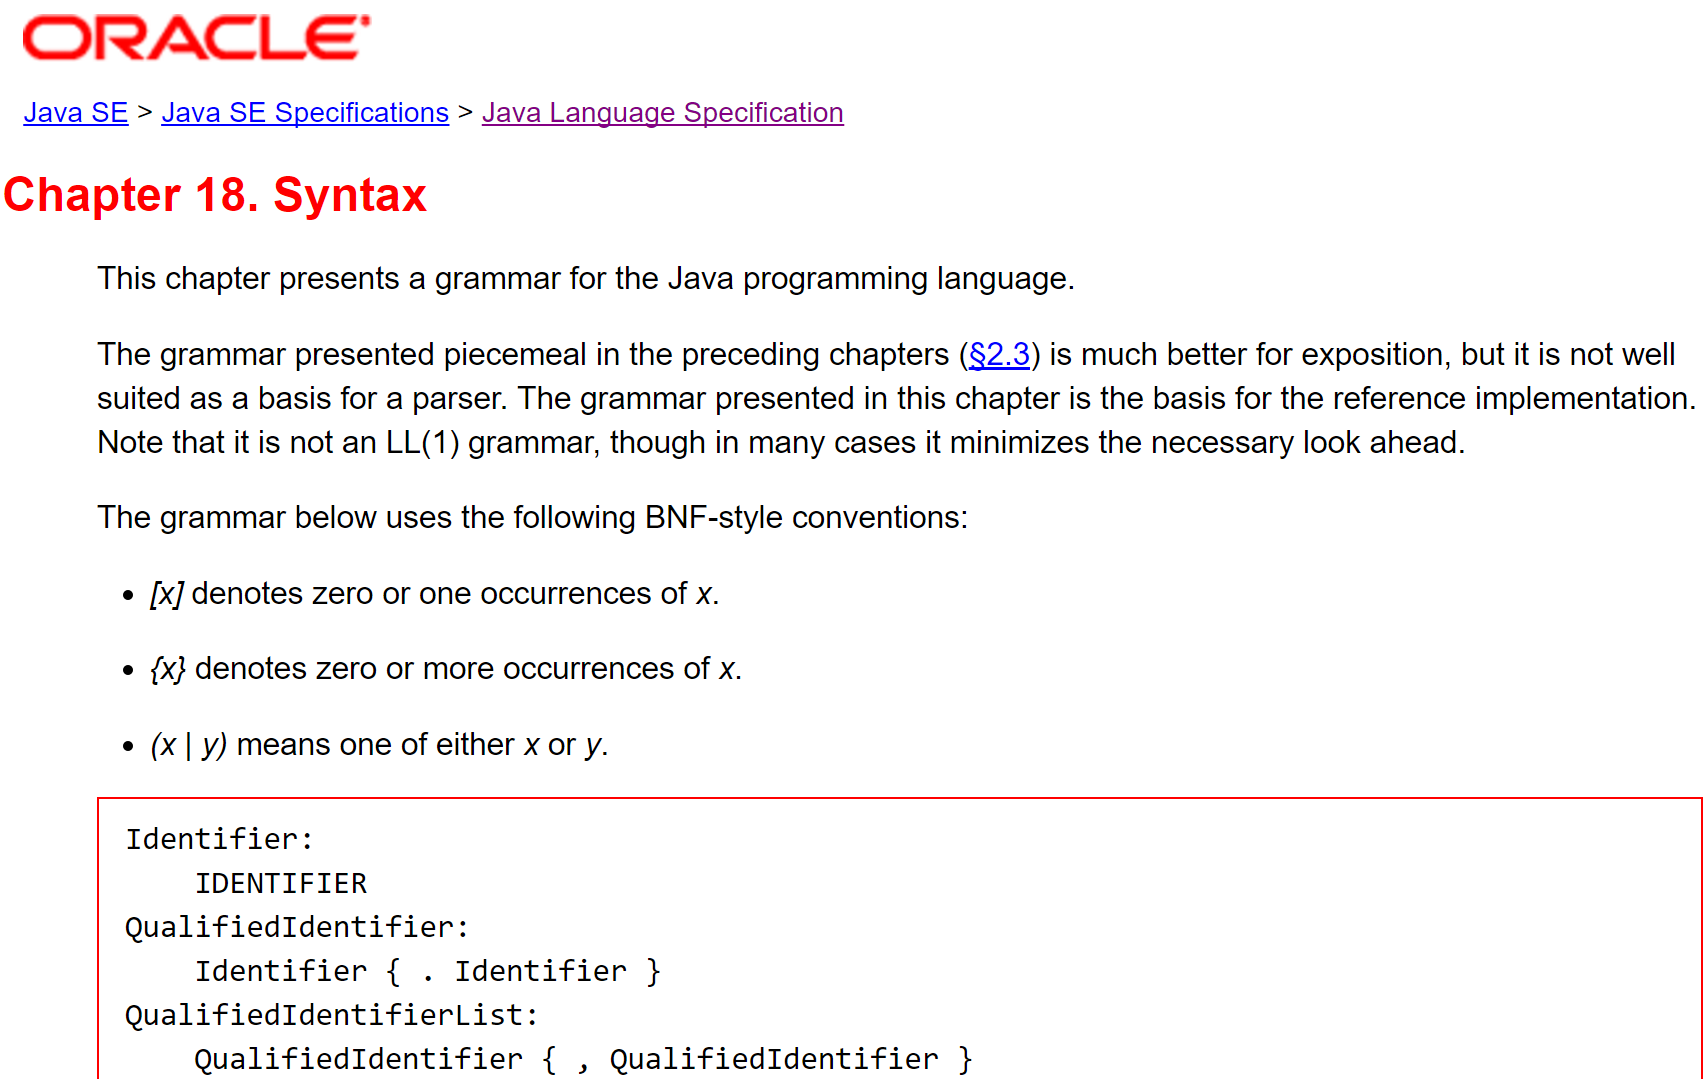
\includegraphics[width=12cm]{pictures/java_grammar.png}} 
%	\end{center}
%\end{frame}
\begin{frame}
     \frametitle{Shuffled Language}
     \only<1>{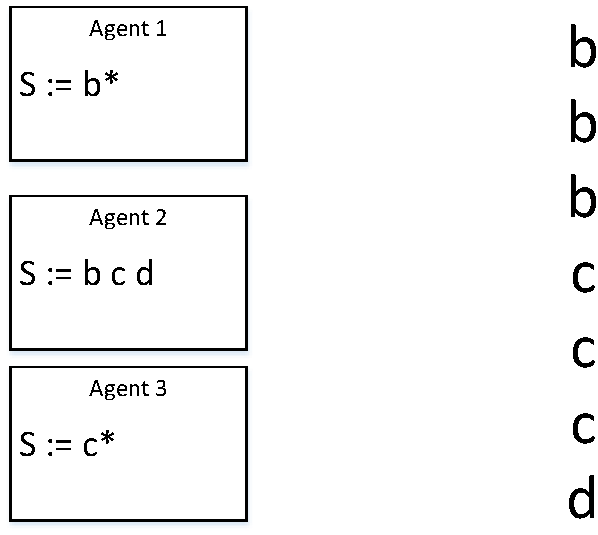
\includegraphics[width=8cm]{pictures/agents.pdf}}
     \only<2-3>{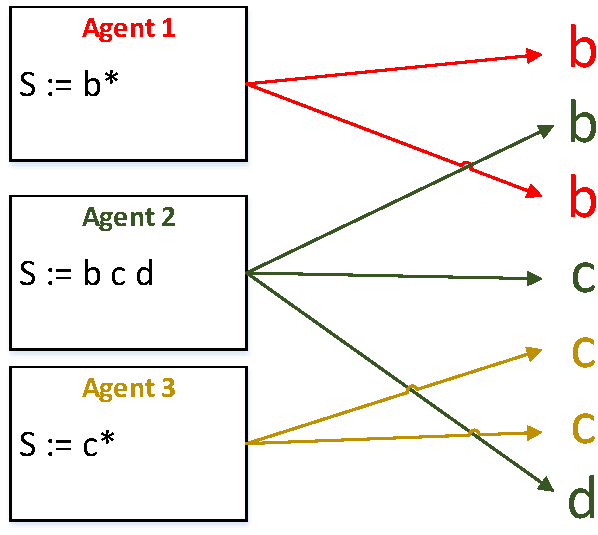
\includegraphics[width=8cm]{pictures/agentsColored.pdf}}
     
     \only<3>{\textbf{Проблема:} Грамматик может быть очень много, а задача NP-полная}
 \end{frame}
 
 \begin{frame}
     \frametitle{Существующие подходы}
         \begin{itemize}
             \item (Maraist, 2016) Generalized LR parsing and the shuffle operator 
             \item Используется GLR
             \item Во время разбора отслеживаются позиции сразу во всех грамматиках
             \item Пространство поиска сужается за счёт поддержания наиболее вероятных веток разбора
             \item Не строятся деревья разбора
         \end{itemize}
 \end{frame}
 
 \begin{frame}
     \frametitle{Наш подход}
     Комбинация синтаксического анализа графов и метода ветвей и границ
 \end{frame}
 
 
 \begin{frame}
     \frametitle{Анализ графов}
     \begin{itemize}
         \item Выделяем все возможные подпоследовательности из входа и обрабатываем как пути в графе
         тут картинка с примером
         \item Для каждой грамматики анализ производится независимо
         \item Результат --- лес разбора всех подпоследовательностей для каждой грамматики
     \end{itemize}
 \end{frame}
 
 \begin{frame}
	\frametitle{Метод ветвей и границ}
	\begin{itemize}
		\item Восстанавливаем входную последовательность по лесам разбора
        тут опять картинка -- дерево B\&B
		\item Отсечение ветви если невозможно взять токен из данного леса
		\item Можно выбирать наиболее вероятную ветку
	\end{itemize}
\end{frame}

 \begin{frame}
    \frametitle{Прогресс работы}
    \begin{itemize}
        \item В поисках данных для адекватного тестирования и сравнения
        \item Планируется публикация
    \end{itemize}
\end{frame}
	%\begin{frame} 
%		\frametitle{Пример постоения леса разбора в оригинальном алгоритме}
%		\begin{columns}
%			\begin{column}{5cm}
%				Вход : \only<1-2>{$\ b c $}
%						\only<3-7>{$\bullet\ b c $} 
%						\only<8-11>{$b\bullet c $}
%						\only<12->{$b c \bullet$} \\
%				\vspace{15pt}
%				Грамматика: \\
%				\vspace{5pt}
%				\only<1>{$$
%					S = \ (a\ |\ b\ |\ S)\ c?
%					$$}
%				\only<2->{$
%				\begin{array}{rl}
%				S =&\only<3,6>{\bullet} \ a\ C\_opt \\
%				|&\only<4,7>{\bullet} \ b\only<8>{\bullet}\ C\_opt \\
%				|&\only<5>{\bullet} \ S\ C\_opt \\
%				C\_opt =& \only<9>{\bullet} \varepsilon \ | \only<10-11>{\bullet} \ c \only<12>{\ \bullet}\\
%				\end{array}
%				$}
%			\end{column}
%			
%			\begin{column}{5cm}
%				\only<3->{
%				\only<8>{\vspace{50pt}}
%				\only<12>{\vspace{44pt}}
%				\begin{center}Очередь дескрипторов\\\end{center}
%				\begin{tabu}{|[3pt]c|[3pt]}
%					\only<10>{$C\_opt =\bullet c$, 1, \dots, \dots \\ \hline}
%					\only<11->{\cellcolor{green!25}{$C\_opt =\bullet c$, 1, \dots, \dots} \\ \hline}
%					\only<11->{\st{$C\_opt =\bullet  \varepsilon$, 1, \dots, \dots} \\ \hline}
%					\only<9-10>{$C\_opt =\bullet  \varepsilon$, 1, \dots, \dots \\ \hline}
%					\only<5-10>{$S =\bullet \ S\ C\_opt$, 0, \dots, \dots \\ \hline}
%					\only<11->{\st{$S =\bullet \ S\ C\_opt$, 0, \dots, \dots} \\ \hline}
%					\only<3-4>{$\ \ \ \ \ \ \ \ \ \ \ \ \ \ \ \ \ \ \ \ \ \ \ \ \ \ \ \ \ \ \ \ \ \ $ \\}
%					%\strike{|[3pt]c|}{quux} & A & B \\
%					\only<4-6>{$S =\bullet \ b\ C\_opt$, 0, \dots, \dots \\ \hline}
%					\only<7-10>{\cellcolor{green!25}{$S =\bullet \ b\ C\_opt$, 0, \dots, \dots} \\ \hline}
%					\only<11->{\st{$S =\bullet \ b\ C\_opt$, 0, \dots, \dots} \\ \hline}
%					\only<3>{$\ \ \ \ \ \ \ \ \ \ \ \ \ \ \ \ \ \ \ \ \ \ \ \ \ \ \ \ \ \ \ \ \ \ $ \\}
%					\only<3-5>{$S =\bullet \ a\ C\_opt$, 0, \dots, \dots}
%					\only<6>{\cellcolor{green!25}{$S =\bullet \ a\ C\_opt$, 0, \dots, \dots}}
%					\only<7->{\st{$S =\bullet \ a\ C\_opt$, 0, \dots, \dots}}
%				\end{tabu}
%			}
		
%			\only<8>{
%				\vspace{20pt}
%				\begin{center}
%					\only<8>{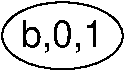
\includegraphics[width=2cm]{pictures/example_trees_b.pdf}}
%				\end{center}				
%			}
%			\only<12>{
%				\begin{center}
%					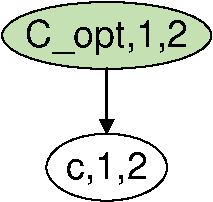
\includegraphics[width=2cm]{pictures/example_trees.pdf}
%				\end{center}				
%			}
%			\end{column}
%		    
%		\end{columns}
%	\end{frame}
\end{document}